% This must be in the first 5 lines to tell arXiv to use pdfLaTeX, which is strongly recommended.
\pdfoutput=1
% In particular, the hyperref package requires pdfLaTeX in order to break URLs across lines.

\documentclass[11pt]{article}

% Remove the "review" option to generate the final version.
\usepackage[review]{acl2023}
% Standard package includes
\usepackage{times}
\usepackage{latexsym}

% For proper rendering and hyphenation of words containing Latin characters (including in bib files)
\usepackage[T1]{fontenc}
% For Vietnamese characters
% \usepackage[T5]{fontenc}
% See https://www.latex-project.org/help/documentation/encguide.pdf for other character sets

% This assumes your files are encoded as UTF8
\usepackage[utf8]{inputenc}
\usepackage{natbib}  % DO NOT CHANGE THIS AND DO NOT ADD ANY OPTIONS TO IT
\usepackage{caption} 
% This is not strictly necessary, and may be commented out,
% but it will improve the layout of the manuscript,
% and will typically save some space.
\usepackage{graphicx}
\usepackage{multirow,array}
\usepackage{bm}
\usepackage{bbm}
\usepackage{algorithm,algorithmicx}
% \usepackage{algorithmic}
\usepackage{amsmath}
\usepackage{amsthm}
\usepackage{verbatim}
\usepackage{booktabs}
\usepackage{amsfonts,amssymb} 
\usepackage[noend]{algpseudocode}
\newcommand{\minitab}[2][l]{\begin{tabular}{#1}#2\end{tabular}}


\newcommand{\secref}[1]{Section \ref{#1}}
\newcommand{\figref}[1]{Figure \ref{#1}}
\newcommand{\eqnref}[1]{Eq. (\ref{#1})}
\newcommand{\tabref}[1]{Table \ref{#1}}
\newcommand{\exref}[1]{Example \ref{#1}}
\newcommand{\KZ}[1]{\textcolor{blue}{Kenny: #1}}


% If the title and author information does not fit in the area allocated, uncomment the following
%
%\setlength\titlebox{<dim>}
%
% and set <dim> to something 5cm or larger.

%\title{Pruning  Pre-trained Language Models with Principled Weight Importance and Self-regularization}

% Author information can be set in various styles:
% For several authors from the same institution:
% \author{Author 1 \and ... \and Author n \\
	%         Address line \\ ... \\ Address line}
% if the names do not fit well on one line use
%         Author 1 \\ {\bf Author 2} \\ ... \\ {\bf Author n} \\
% For authors from different institutions:
% \author{Author 1 \\ Address line \\  ... \\ Address line
	%         \And  ... \And
	%         Author n \\ Address line \\ ... \\ Address line}
% To start a seperate ``row'' of authors use \AND, as in
% \author{Author 1 \\ Address line \\  ... \\ Address line
	%         \AND
	%         Author 2 \\ Address line \\ ... \\ Address line \And
	%         Author 3 \\ Address line \\ ... \\ Address line}

%\author{First Author \\
	%	Affiliation / Address line 1 \\
	%	Affiliation / Address line 2 \\
	%	Affiliation / Address line 3 \\
	%	\texttt{email@domain} \\\And
	%	Second Author \\
	%	Affiliation / Address line 1 \\
	%	Affiliation / Address line 2 \\
	%	Affiliation / Address line 3 \\
	%	\texttt{email@domain} \\}

\begin{document}
	\appendix
	\section{Results with More PLMs on subset of GLUE}
	In addition the widely used BERT and GPT-2 models, we also perform pruning experiments upon other two pre-trained language models: Electra$_{\text{base}}$ and MiniLM$_{\text{12L-384H}}$ to further verify the effectiveness of our method. 
	
	Due to computing resource constraint, we restrict our experiments on a subset of GLUE task, including RTE, CoLA and QNLI at 80\% and 90\% sparsity. We compare PINS against IMP and PLATON as two representative baselines for magnitude-based and sensitivity-based pruning methods. We fix the batch size as 32 and learning rate as 3e-5 similar to the BERT experiments. We illustrate the pruning results on \tabref{table:electra} and \tabref{table:minilm}. At both sparsity levels, PINS consistently outperforms IMP and PLATON on all three datasets, verifying the general effectiveness of PINS for language model pruning.
	\begin{table}[h]
		\centering
%		\normalsize
		\small
		\begin{tabular}{c|l|ccc}
			\toprule
			\multirow{2}{*}{Sparsity} & \multicolumn{1}{c|}{\multirow{2}{*}{Method}} & \multicolumn{1}{c}{\multirow{2}{*}{\begin{tabular}[c]{@{}c@{}}\textbf{RTE}\\ Acc\end{tabular}}} & \multicolumn{1}{c}{\multirow{2}{*}{\begin{tabular}[c]{@{}c@{}}\textbf{CoLA}\\ Mcc\end{tabular}}} & \multicolumn{1}{c}{\multirow{2}{*}{\begin{tabular}[c]{@{}c@{}}\textbf{QNLI}\\ Acc\end{tabular}}} \\
			& \multicolumn{1}{c|}{}                        & \multicolumn{1}{c}{}                                                                   & \multicolumn{1}{c}{}                                                                   & \multicolumn{1}{c}{}                                                                                                                              \\
			\midrule
			\multicolumn{1}{c|}{0\%}   & Fine-tune                                  & 73.0                                                                                  &58.5
			                                                                                 &91.5                                                                                                                                                                                                                                                                                 \\
			\midrule
			\multirow{3}{*}{80\%}     &IMP                                                &60.5                                                                                       &   21.6                                                                                     &   87.5                                                                                               \\
			&PLATON                                            &  68.2                                                                                      &  54.1                                                                                      &     89.8                                                                                           \\
			&PINS~(ours)                                             &   69.5                                                                                   &      54.4                                                                                 &  90.4                                                                                          \\
			\midrule
			\multirow{3}{*}{90\%}     &IMP                                              &   57.5                                                                                    &   14.1                                                                                     &   83.9                                                                                     \\
			& PLATON                                               &   63.1                                                                                   &  38.8                                                                                      &  88.0                                                                                        \\
			&PINS~(ours)                                             &   66.2                                                                                    &     44.8                                                                                  &   88.6                                                                                  \\
			\bottomrule                                     
		\end{tabular}
		\caption{Results with MiniLM$_{\text{12L-384H}}$ on the GLUE development set.}
		\label{table:electra}
	\end{table}
	\begin{table}[h]
	\centering
%	\normalsize
	\small
	\begin{tabular}{c|l|ccc}
		\toprule
		\multirow{2}{*}{Sparsity} & \multicolumn{1}{c|}{\multirow{2}{*}{Method}} & \multicolumn{1}{c}{\multirow{2}{*}{\begin{tabular}[c]{@{}c@{}}\textbf{RTE}\\ Acc\end{tabular}}} & \multicolumn{1}{c}{\multirow{2}{*}{\begin{tabular}[c]{@{}c@{}}\textbf{CoLA}\\ Mcc\end{tabular}}} & \multicolumn{1}{c}{\multirow{2}{*}{\begin{tabular}[c]{@{}c@{}}\textbf{QNLI}\\ Acc\end{tabular}}} \\
		& \multicolumn{1}{c|}{}                        & \multicolumn{1}{c}{}                                                                   & \multicolumn{1}{c}{}                                                                   & \multicolumn{1}{c}{}                                                                                                                                   \\
		\midrule
		\multicolumn{1}{c|}{0\%}   & Fine-tune                                  &  81.9                                                                                 &69.0
		&  93.1                                                                                                                                                                   \\
		\midrule
		\multirow{3}{*}{80\%}     &IMP                                                & 59.9                                                                                      &    11.2                                                                                    &  87.5                                                                                          \\
		&PLATON                                            &  73.6                                                                                      &    60.0                                                                                    & 91.0                                                                                        \\
		&PINS~(ours)                                             &    75.5                                                                                  &      63.7                                                                                 &  92.0                                                                                     \\
		\midrule
		\multirow{3}{*}{90\%}     &IMP                                              &   52.9                                                                                    &0.0                                                                                        &    83.0                                                                                 \\
		& PLATON                                               &  69.9                                                                                    &    48.0                                                                                    &   89.7                                                                                   \\
		&PINS~(ours)                                             &  72.3                                                                                     &     49.2                                                                                  &      90.2                                                                                \\
		\bottomrule                                     
	\end{tabular}
	\caption{Results with Electra$_{\text{base}}$ on the GLUE development set.}
	\label{table:minilm}
\end{table}

\section{Proof of Theorem 1}
%Proof of Theorem 1:
\begin{proof}
		Let $t_i$ and $t_{j}$ where $t_{i}\geq t_{j}$ denote the time steps at which two different checkpoints are saved; Let $R(f_{\bm{\theta}^{(t\leftarrow t_i)}})$ and $R(f_{\bm{\theta}^{(t\leftarrow t_j)}})$ denote the expected generalization error of models learned from  $f_{\bm{\theta}^{(t_i)}}$ and $f_{\bm{\theta}^{(t_j)}}$; Let $n$ denotes the size of training data; $|\cdot|_{\text{C}}$ denotes a capacity measure like VC-dimension for function class $\mathcal{F}_{\bm{\theta}}$. Based on previous expositions on VC theory, the following asymptotic generalization bound holds:
	\begin{align}\nonumber
		R(f_{\bm{\theta}^{(t\leftarrow t_i)}})&=R(f_{\bm{\theta}^{(t\leftarrow t_i)}})-R(f_{\bm{\theta}^{(t_i)}})+R(f_{\bm{\theta}^{(t_i)}}) \\ \nonumber
		&\leq O(\frac{|\mathcal{F}_{\bm{\theta}^{(t)}}|_{\text{C}}}{n^{\alpha_{i}}})+ \epsilon_{t,t_i} + R(f_{\bm{\theta}^{(t_i)}}) \\ \nonumber 
		&=  \underbrace{O(\frac{|\mathcal{F}_{\bm{\theta}^{(t)}}|_{\text{C}}}{n^{\alpha_{i}}}) + \underset{f_{\bm{\theta}^{(t)}}\in \mathcal{F}_{\bm{\theta}^{(t\leftarrow t_i)}}}{\inf}R(f_{\bm{\theta}^{(t)}})}_{bound(f_{\bm{\theta}^{(t\leftarrow t_i)}})} \\ \nonumber
		R(f_{\bm{\theta}^{(t\leftarrow t_j)}})&=R(f_{\bm{\theta}^{(t\leftarrow t_j)}})-R(f_{\bm{\theta}^{(t_j)}})+R(f_{\bm{\theta}^{(t_j)}}) \\ \nonumber
		&\leq O(\frac{|\mathcal{F}_{\bm{\theta}^{(t)}}|_{\text{C}}}{n^{\alpha_{j}}})+ \epsilon_{t,t_j} + R(f_{\bm{\theta}^{(t_j)}}) \\ \nonumber 
		&=  \underbrace{O(\frac{|\mathcal{F}_{\bm{\theta}^{(t)}}|_{\text{C}}}{n^{\alpha_{j}}}) + \underset{f_{\bm{\theta}^{(t)}}\in \mathcal{F}_{\bm{\theta}^{(t\leftarrow t_j)}}}{\inf}R(f_{\bm{\theta}^{(t)}})}_{bound(f_{\bm{\theta}^{(t\leftarrow t_j)}})}
	\end{align}
	where $\epsilon_{t,ti}$ is the approximation error of function class $\mathcal{F}_{\bm{\theta}^{(t\leftarrow t_i)}}$ with respect to $f_{\bm{\theta}^{(t_i)}}$. $\epsilon_{t,tj}$ is defined in analogy.
	Because: (1) $\bm{\theta}^{(t_i)}$ is a later checkpoint with higher sparsity than $\bm{\theta}^{(t_j)}$, we have the learning speed $1\geq \alpha_{i}\geq \alpha_{j}\geq \frac{1}{2}$; (2) $f_{\bm{\theta}^{(t_i)}}$ has lower generalization error than $f_{\bm{\theta}^{(t_j)}}$, we have the following inequality holds with high probability:
	\begin{align}\nonumber
		bound(f_{\bm{\theta}^{(t\leftarrow t_i)}}) \leq bound(f_{\bm{\theta}^{(t\leftarrow t_j)}})
	\end{align}
\end{proof}
\newtheorem{theorem}{Theorem}
%\begin{theorem}
%	Let $t_i$ and $t_{j}$ where $t_{i}\geq t_{j}$ denote the time steps at which two different checkpoints are saved; Let $R(f_{\bm{\theta}^{(t\leftarrow t_i)}})$ and $R(f_{\bm{\theta}^{(t\leftarrow t_j)}})$ denote the expected generalization error of models learned from two checkpoints $\bm{\theta}^{(t_i)}$ and $\bm{\theta}^{(t_j)}$; Let n denotes the size of training data; $|\cdot|_{\text{C}}$ denotes a function class capacity measure like VC-dimension. Based on previous expositions on VC theory, the following asymptotic generalization bound holds:
%	\begin{align}\nonumber
%		R(f_{\bm{\theta}^{(t\leftarrow t_i)}})&=R(f_{\bm{\theta}^{(t\leftarrow t_i)}})-R(f_{\bm{\theta}^{(t_i)}})+R(f_{\bm{\theta}^{(t_i)}}) \\ \nonumber
%				&\leq O(\frac{|f_{\bm{\theta}^{(t)}}|_{\text{C}}}{n^{\alpha_{i}}})+ \epsilon_{t,t_i} + R(f_{\bm{\theta}^{(t_i)}}) \\ \nonumber 
%				&=  \underbrace{O(\frac{|f_{\bm{\theta}^{(t)}}|_{\text{C}}}{n^{\alpha_{i}}}) + \underset{\bm{\theta}^{(t)}\in \mathcal{F}_{\bm{\theta}^{(t\leftarrow t_i)}}}{\inf}R(f_{\bm{\theta}^{(t)}})}_{bound(f_{\bm{\theta}^{(t\leftarrow t_i)}})} \\ \nonumber
%		R(f_{\bm{\theta}^{(t\leftarrow t_j)}})&=R(f_{\bm{\theta}^{(t\leftarrow t_j)}})-R(f_{\bm{\theta}^{(t_j)}})+R(f_{\bm{\theta}^{(t_j)}}) \\ \nonumber
%&\leq O(\frac{|f_{\bm{\theta}^{(t)}}|_{\text{C}}}{n^{\alpha_{j}}})+ \epsilon_{t,t_j} + R(f_{\bm{\theta}^{(t_j)}}) \\ \nonumber 
%&=  \underbrace{O(\frac{|f_{\bm{\theta}^{(t)}}|_{\text{C}}}{n^{\alpha_{j}}}) + \underset{\bm{\theta}^{(t)}\in \mathcal{F}_{\bm{\theta}^{(t\leftarrow t_j)}}}{\inf}R(f_{\bm{\theta}^{(t)}})}_{bound(f_{\bm{\theta}^{(t\leftarrow t_j)}})}
%	\end{align}
%where $\epsilon_{t,ti}$ is the approximation error of function class $\mathcal{F}_{\bm{\theta}^{(t\leftarrow t_i)}}$ with respect to $f_{\bm{\theta}^{(t_i)}}$. $\epsilon_{t,tj}$ is defined in analogy.
%	Because: (1) $\bm{\theta}^{(t_i)}$ is a later checkpoint with higher sparsity than $\bm{\theta}^{(t_j)}$, we have the learning speed $1\geq \alpha_{i}\geq \alpha_{j}\geq \frac{1}{2}$; (2) $\bm{\theta}^{(t_i)}$ has lower generalization error than $\bm{\theta}^{(t_j)}$, we have the following inequality holds with large probability:
%	\begin{align}\nonumber
%		bound(f_{\bm{\theta}^{(t\leftarrow t_i)}}) \leq bound(f_{\bm{\theta}^{(t\leftarrow t_j)}})
%	\end{align}
%\end{theorem}

\begin{figure*}[t]
	\centering
	\scalebox{0.48}{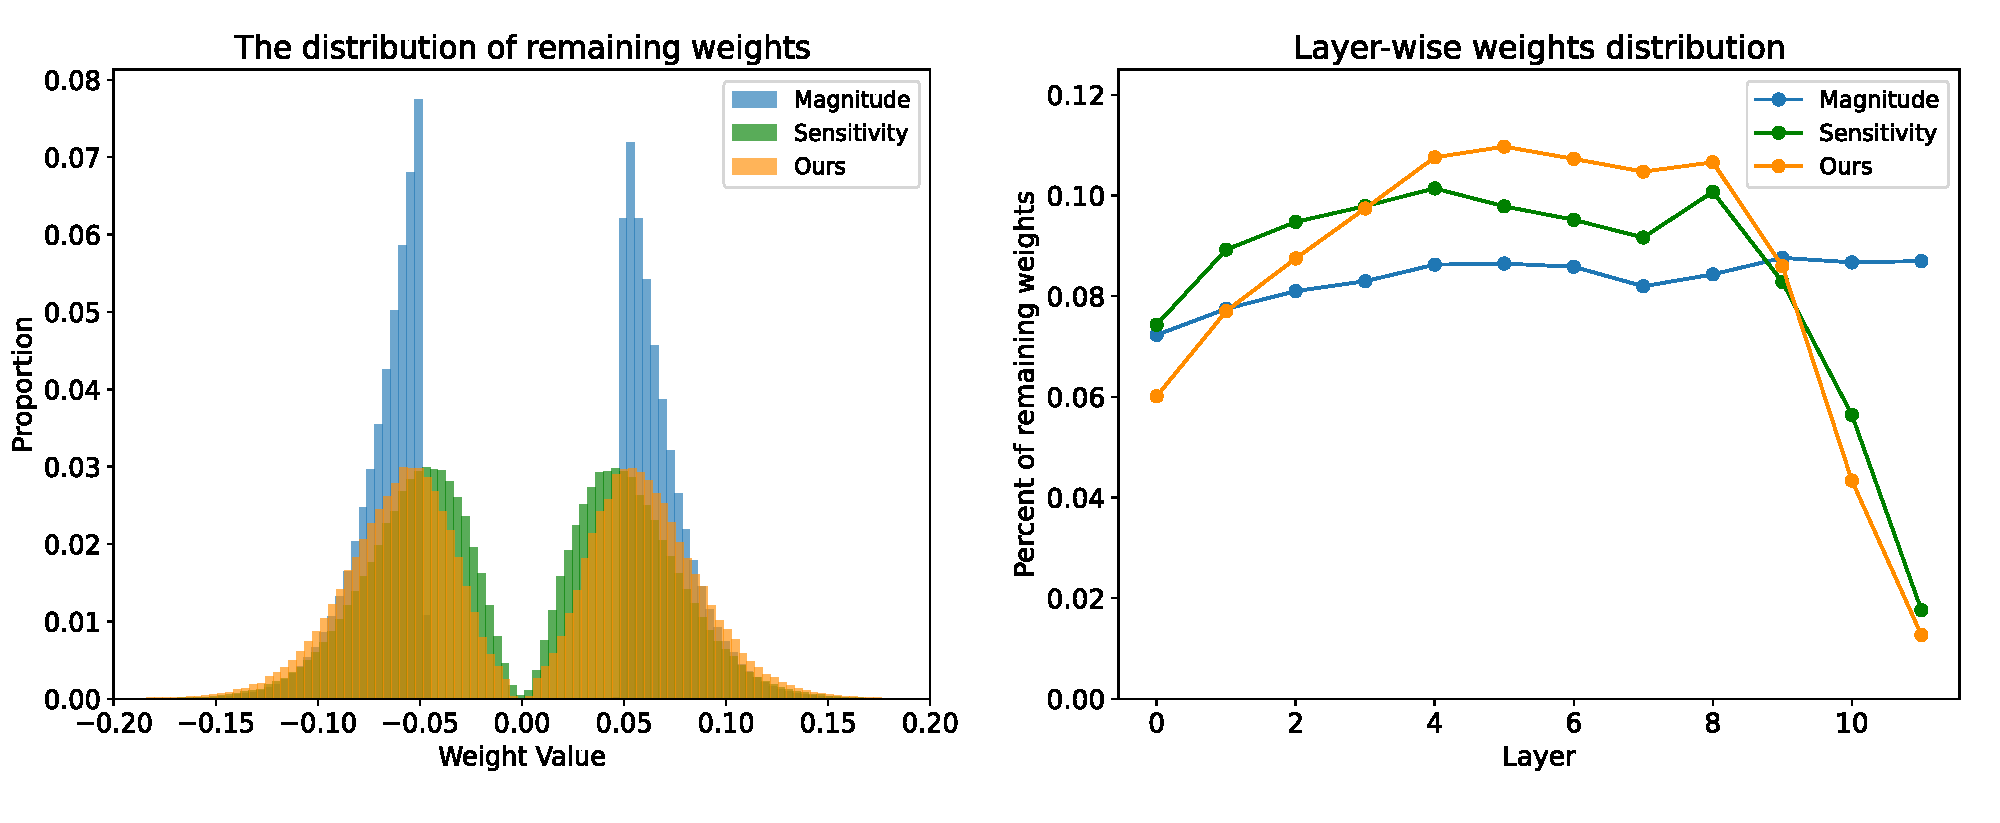
\includegraphics{./figures/weights_stats.pdf}}
	\caption{Weight distributions of BERT$_{\text{base}}$ pruned using different importance criteria on RTE dataset. Left figure shows the value distribution and the right figure shows how remaining parameters are distributed at different model layers.}
	\label{fig:intersim}
\end{figure*}
\begin{figure}[t]
	\centering
	\scalebox{0.355}{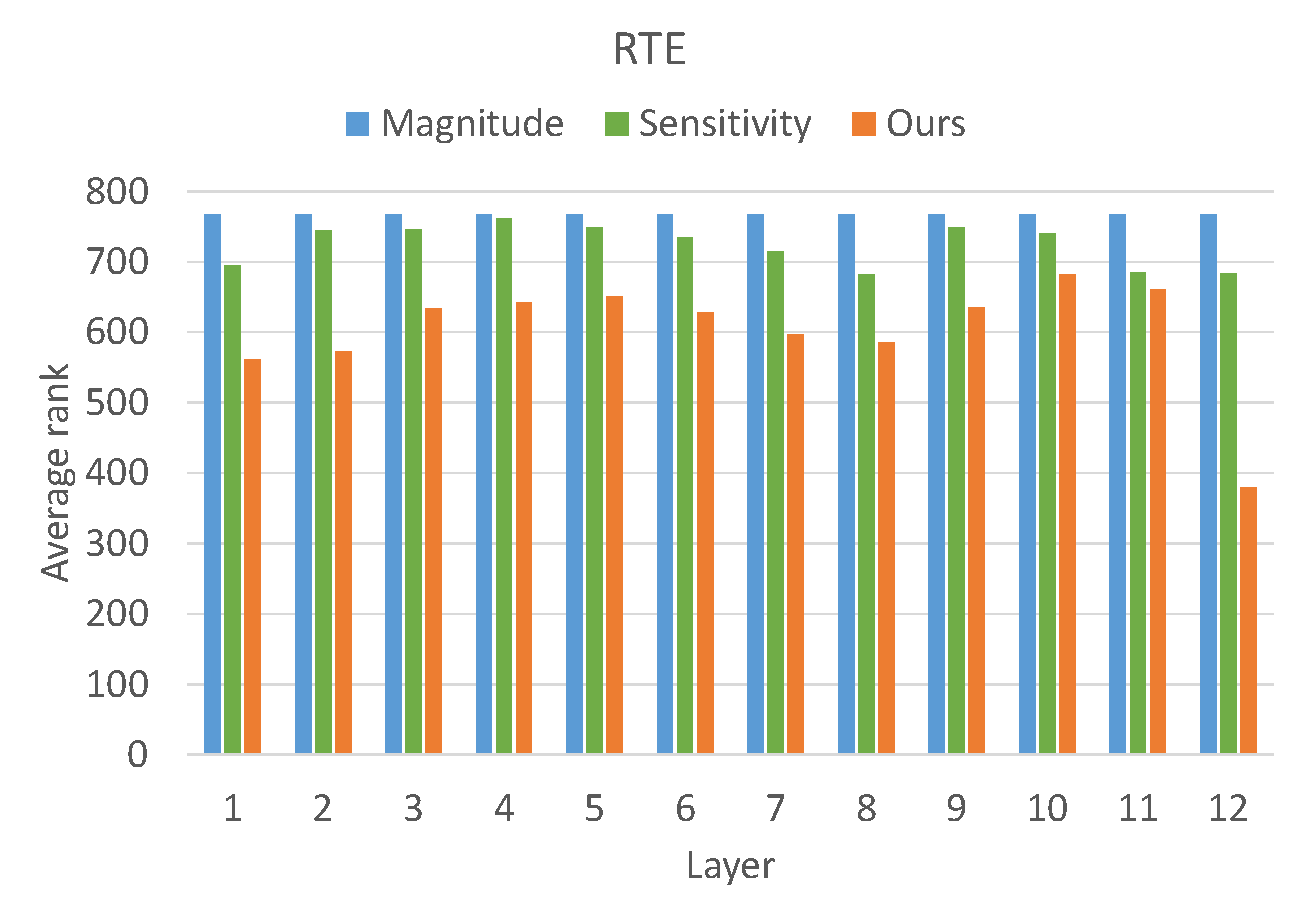
\includegraphics{./figures/rank_dist_rte.pdf}}
	\caption{Layerwise rank distribution of BERT$_{\text{base}}$ pruning using different importance criteria on RTE dataset.}
	\label{fig:rank_dist}
\end{figure}

\section{More Post-pruning Analyses}
This section presents more visualized analyses of models sparsified by different pruning methods. 

\figref{fig:rank_dist} shows the layerwise rank distribution of BERT$_{\text{base}}$ pruned using different importance criteria on the RTE dataset. The observation here is similar to what is discussed in the main body of the paper: PINS exhibits the lowest average matrix rank in the sparsified model compared to the other two criteria.

\figref{fig:intersim} illustrates the weight distribution of BERT$_{\text{base}}$ pruning using different importance criteria. From the left figure we can see that magnitude-based pruning tends to keep parameters with high absolute values, which is expected based on its definition. Sensitivity and PINS produce similar weight value distribution mainly because the two methods both contain the $g\theta$ term in their importance calculation. Despite the similarity, we can still observe that PINS produces smoother distribution than sensitivity and covers more weights with larger absolute values. 


The right figure shows the layerwise distribution of remaining parameters after pruning. A clear trend is that PINS tends to retain more parameters in the middle layers~(4-7), which also coincided with the inter-model sparsity pattern analysis in the main body of our paper. Both sensitivity and PINS remove a large proportion of parameters in the top layers~(10-12) while magnitude-based pruning has no preference for model layers.




\section{Sparsity Scheduler}
The proportion of remaining weights is controlled by the sparsity scheduler, here  we adopt the commonly used  cubic sparsity schedule to progressively reach target sparsity, i.e., $v^{(t)}$ at time step $t$ within the maximum time steps $T$ is given by:
\begin{align}
	%	v^{(t)}=
	\begin{cases} 
		v_i & t\in [0, t_i) \\
		v_f+(v_i-v_f)(\frac{T-t_{f}-t}{T-t_f-t_i})^3 & t\in[t_i, T-t_f) \\
		v_f  & \text{otherwise}  
	\end{cases}
\end{align}
\label{eq:prune}
where $v_i=1.0$, $v_f$ is the final percent of remained parameters, $t_i$ and $t_f$ are the warmup and cool-down steps.

\section{Accelerating Inference and Reducing Storage}
We attain practical efficiency gain in terms of inference time and disk storage space using different sets of off-the-shelf techniques. Specifically, we use DeepSparse\footnote{\url{https://github.com/neuralmagic/deepsparse}}, a sparsity-aware inference runtime to accelerate inference of sparse model on CPUs. We also utilize the Pytorch built-in quantization function\footnote{\url{https://pytorch.org/docs/stable/quantization.html}} and Compressed Sparse Row~(CSR) format\footnote{\url{https://github.com/huggingface/block_movement_pruning/blob/master/Saving_PruneBERT.ipynb}} to achieve a much smaller disk space requirement.
	% Entries for the entire Anthology, followed by custom entries
	% \bibliography{anthology,custom}
	
	%	
	%	\clearpage
	%	\section{Depression Templates}

\begin{table}[htbp]
  \small
  \centering
  \begin{tabular}{l|l}
  \hline
  Dimension & Template \\
  \hline
  Feeling Depressed  &  I feel depressed. \\
  Diagnosis &  I am diagnosed with depression. \\
  Treatment &  I am treating my depression. \\
  \hline
  Sadness & I feel sad.  \\
  Pessimism & I am discouraged about my future.  \\
  Past Failure & I always fail. \\
  Loss of Pleasure & I don't get pleasure from things. \\
  Guilty Feelings & I feel quite guilty. \\
  Punishment Feelings & I expected to be punished. \\
  Self-Dislike & I am disappointed in myself. \\
  Self-Criticalness & I always criticize myself for my faults. \\
  Suicidal Thoughts or Wishes & I have thoughts of killing myself. \\
  Crying & I always cry. \\
  Agitation & I am hard to stay still. \\
  Loss of Interest & It's hard to get interested in things. \\
  Indecisiveness & I have trouble making decisions. \\
  Worthlessness & I feel worthless. \\
  Loss of Energy & I don't have energy to do things. \\
  Changes in Sleeping Pattern & I have changes in my sleeping pattern. \\
  Irritability & I am always irritable. \\
  Changes in Appetite & I have changes in my appetite. \\
  Concentration Difficulty & I feel hard to concentrate on things. \\
  Tiredness  & I am too tired to do things. \\
  Loss of Interest in Sex & I have lost my interest in sex. \\
  \hline
  \end{tabular}
  \caption{The main templates and their corresponding dimensions we used in our experiments, including 3 direct depression descriptions and 21 indirect symptoms derived from BDI-II \citep{beck1996beck}. }
  \label{table:bdi}
\end{table}


We provide the complete templates in Table \ref{table:bdi}. We mainly use a combination of 3 direct depression descriptions and the 21 indirect symptoms derived from BDI-II. We also experimented other well-known depression scales like HDRS \citep{hamilton1986hamilton}, CES-D \citep{Lenore1977CES-D} and PHQ-9 \citep{kroenke2001phq} (We will release our revised templates for theses scales along with our code). The original scales usually contain different descriptions under the same dimension to distinguish different level of intensity or frequency. However, we find that current sentence representations have difficulty in capturing such nuanced differences. We thus condense the descriptions of each dimension into one general template (A few may have more, if there are significant intra-dimension difference).

\end{document}
